\section{Derivation of trinormal closures by transformation of binormal closures}
\label{sec:derivation-of-trinormal-closures-by-transformation-of-binormal-closures}

Analytic closures between higher and lower order moments for the binormal case
are available (see~CLUBB-SILHS\autocite{larson2022clubbsilhs}).
We wish to derive similar analytic closures for the proposed trinormal \gls{pdf}.
Deriving an analytic closure for a general trinormal \gls{pdf} is difficult.
However, doing so is tractable in the special case that the third normal component
is located at the mean of the binormal \gls{pdf}.
In fact, the trinormal closures can be derived
by making a simple transformation of the binormal closures~\cite{larson2005using},
e.g.
\begin{align}
    \label{eq:wp2_bar_dGn}
    \wptwo
    &= \alpha [(w_1 - \overline{w})^2 + \sigma_w^2]
    + (1 - \alpha) [(w_2 - \overline{w})^2 + \sigma_w^2].
\end{align}
This section will demonstrate that the following transformations,
denoted by the subscript \enquote{dGn} for the binormal case,
successfully achieve this conversion.
\begin{align}
    \label{eq:w_prime_2_transform}
    \overline{w'^2} \frac{1 - \delta\lambda_w}{1 - \delta}
    &= \overline{w'^2}_{dGn},
\end{align}
\begin{align}
    \label{eq:w_prime_3_transform}
    \overline{w'^3} \frac{1}{1 - \delta}
    &= \overline{w'^3}_{dGn},
\end{align}
\begin{align}
    \label{eq:w_prime_3_div_w_prime_2_transform}
    \frac{\overline{w'^3}}{\overline{w'^2}^{3/2}} \frac{(1 - \delta)^{1/2}}{(1 - \lambda_w\delta)^{3/2}}
    &= \frac{\overline{w'^3}_{dGn}}{\overline{w'^2}_{dGn}^{3/2}},
\end{align}
\begin{align}
    \label{eq:theta_l_prime_transform}
    \overline{\theta_l'^2} \frac{1 - \delta\lambda_\theta}{1 - \delta}
    &= \overline{\theta_l'^2}_{dGn},
\end{align}
\begin{align}
    \label{eq:w_prime_theta_l_prime_transform}
    \overline{w'\theta_l'} \frac{1 - \delta\lambda_{w\theta}}{1 - \delta}
    &= \overline{w'\theta_l'}_{dGn},
\end{align}
\begin{align}
    \label{eq:w_prime_4_transform}
    \left(\overline{w'^4} - 3\delta\lambda_w^2 \left(\overline{w'^2}\right)^2\right) \frac{1}{1 - \delta}
    &= \overline{w'^4}_{dGn}
\end{align}
\begin{align}
    \label{eq:w_prime_4_div_w_prime_2_transform}
    \left(\frac{\overline{w'^4}}{(\overline{w'^2})^2} - 3\delta\lambda_w^2 \right) \frac{1 - \delta}{(1 - \lambda_w\delta)^2}
    &= \frac{\overline{w'^4}_{dGn}}{(\overline{w'^2}_{dGn})^2}
\end{align}
To get a sense of what those transformations mean and why they should work,
we pick e.g. \cref{eq:w_prime_2_transform}.
If we substitute in the already defined formula for $\lambda_w$ (\cref{eq:lambda}), we get
\begin{align}
    \overline{w'^2} \left(1 - \delta\frac{\sigma_{w 3}^2}{\wptwo}\right)
    &= (1 - \delta)\overline{w'^2}_{dGn} \nonumber\\
    \overline{w'^2} - \delta\sigma_{w 3}^2
    &= (1 - \delta)\overline{w'^2}_{dGn} \nonumber\\
    \overline{w'^2}
    &= \overline{w'^2}_{dGn} - \delta\overline{w'^2}_{dGn} + \delta\sigma_{w 3}^2 \nonumber\\
    \overline{w'^2}
    &= \overline{w'^2}_{dGn} - \delta\left(\overline{w'^2}_{dGn} - \sigma_{w 3}^2\right).
\end{align}
Our analysis reveals a key relationship between the parameter $\delta$
and the overall variance (often referred to as \enquote{width}) of the trinormal distribution.
As the value of $\delta$ approaches 1 (but strictly remains less than 1),
the standard deviation of the third normal distribution
has a progressively stronger influence on the overall variance of the combined distribution.
This intuitively makes sense because a larger weight assigned to the third normal distribution through $\delta$
will contribute more significantly to the spread of the combined \gls{pdf}.

Also, if we look at \cref{eq:w_prime_3_transform}, we see that there is no more $\lambda_w$ present.
It makes sense graphically, that as $\delta$ grows,
which means that the normal \gls{pdf} in the middle is growing,
the overall skewness of all three normals has to change also,
depending on the value of $\sigma_{w 3}$.
We can see this, as well as the relationship between the variance in \cref{tab:1dplotbitri}.
\begin{table}[!htb]
    \centering
    \begin{tabularx}{\textwidth}{c|@{}Y@{}@{}Y@{}@{}Y@{}}
        \diagbox{$\sigma_{w 3}$}{$\delta$} & 0.1 & 0.5 & 0.9 \\
        \hline
        0.5
        & 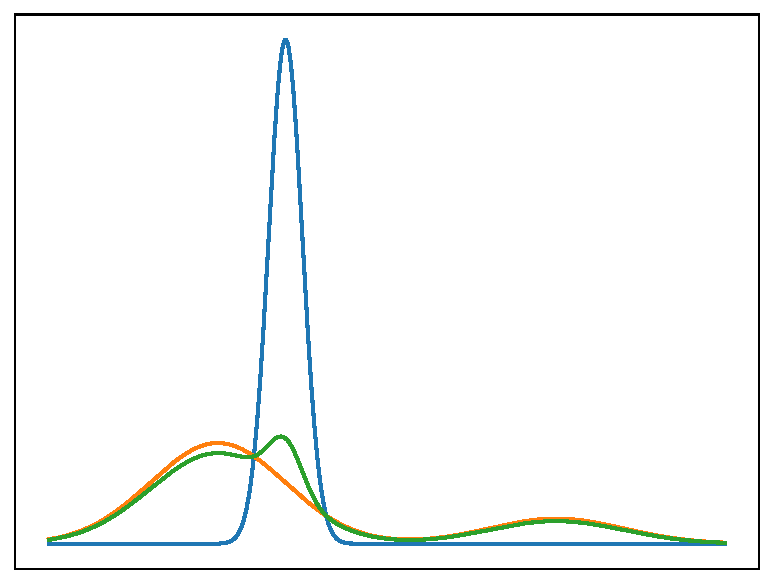
\includegraphics[width = .29\textwidth]{include/figures/1dplotslw5_delta1}
        & 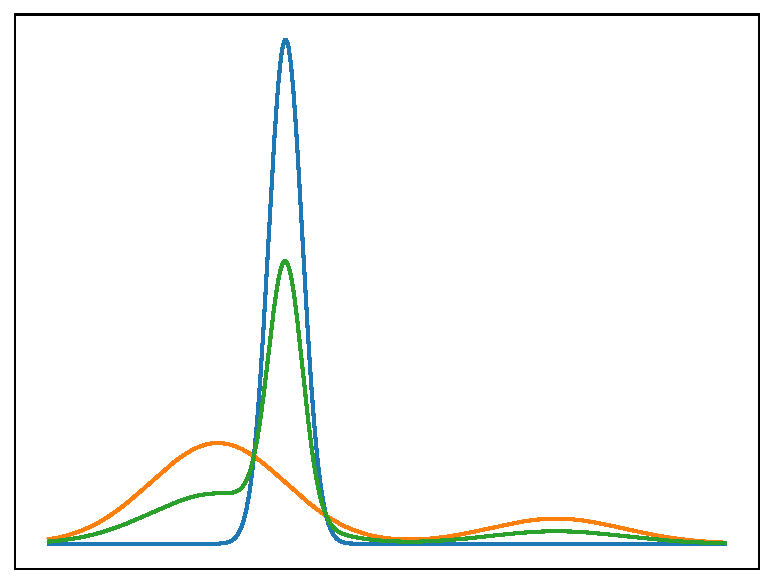
\includegraphics[width = .29\textwidth]{include/figures/1dplotslw5_delta5}
        & 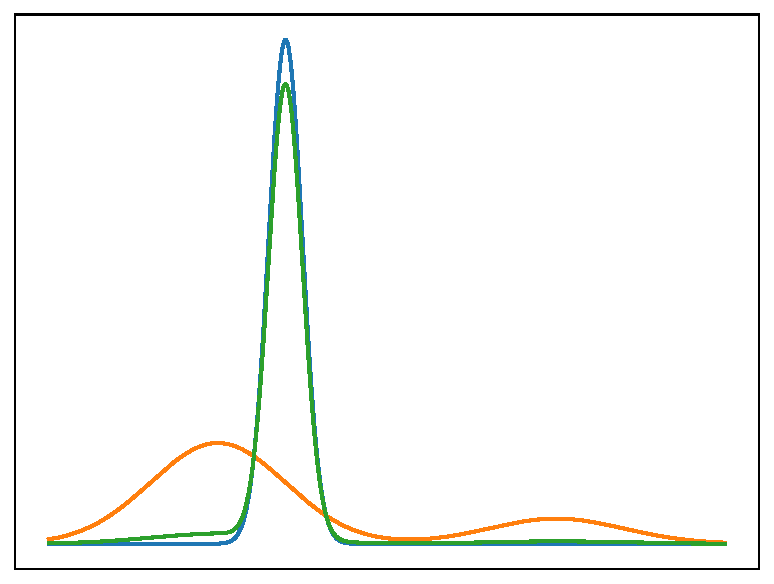
\includegraphics[width = .29\textwidth]{include/figures/1dplotslw5_delta9} \\
        \hline
        4
        & 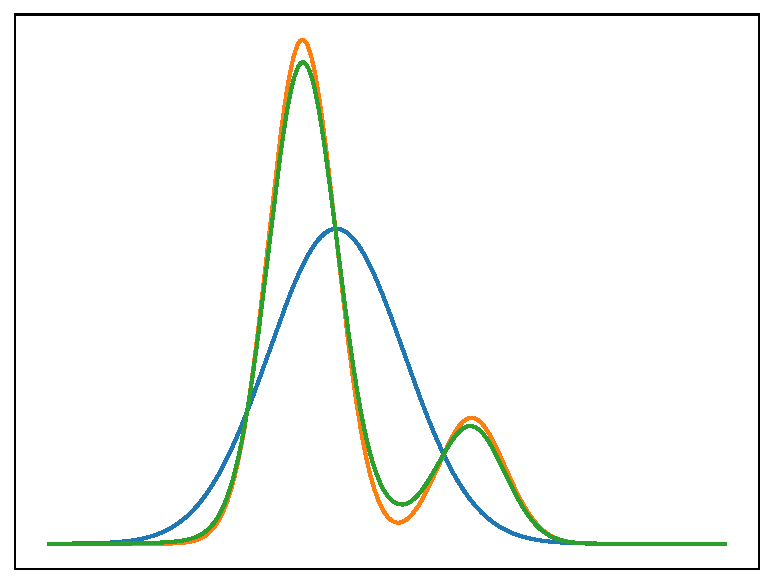
\includegraphics[width = .29\textwidth]{include/figures/1dplotslw40_delta1}
        & 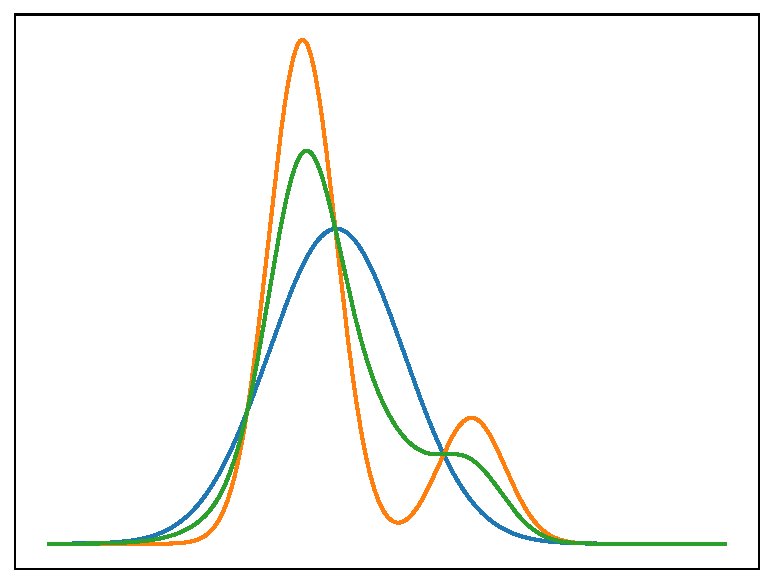
\includegraphics[width = .29\textwidth]{include/figures/1dplotslw40_delta5}
        & 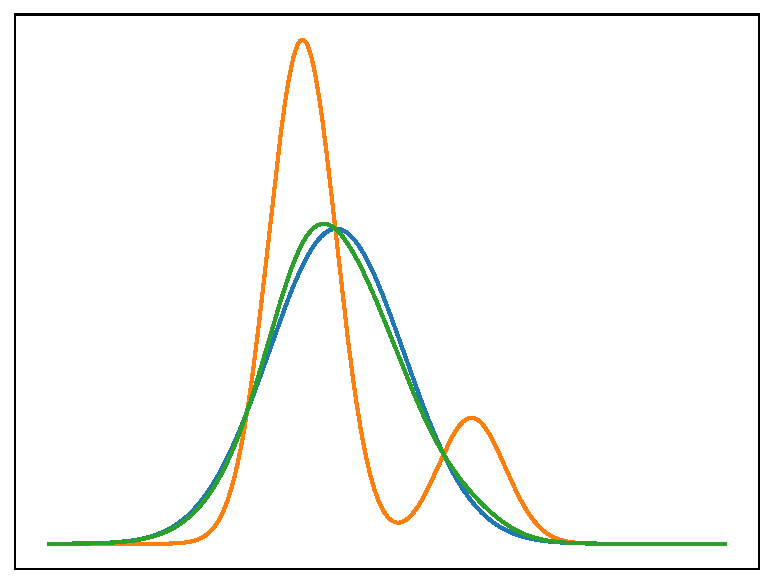
\includegraphics[width = .29\textwidth]{include/figures/1dplotslw40_delta9} \\
        \hline
        8
        & 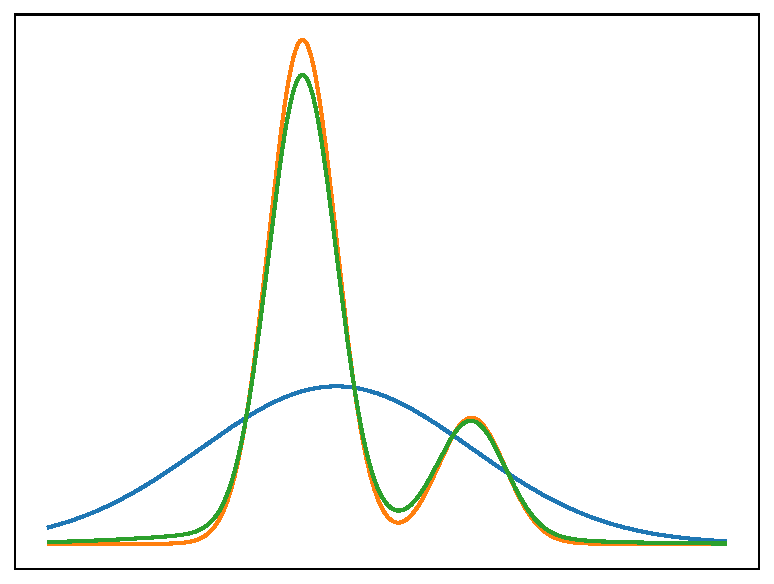
\includegraphics[width = .29\textwidth]{include/figures/1dplotslw80_delta1}
        & 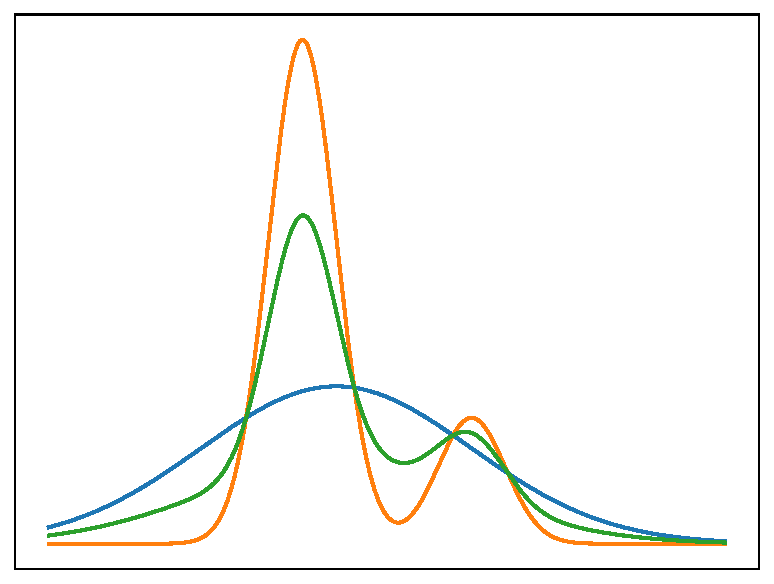
\includegraphics[width = .29\textwidth]{include/figures/1dplotslw80_delta5}
        & 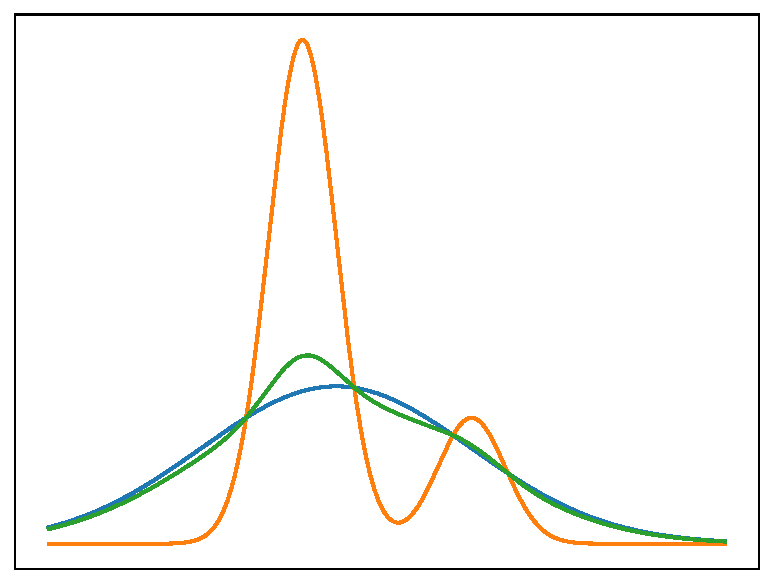
\includegraphics[width = .29\textwidth]{include/figures/1dplotslw80_delta9} \\
        \hline
        10
        & 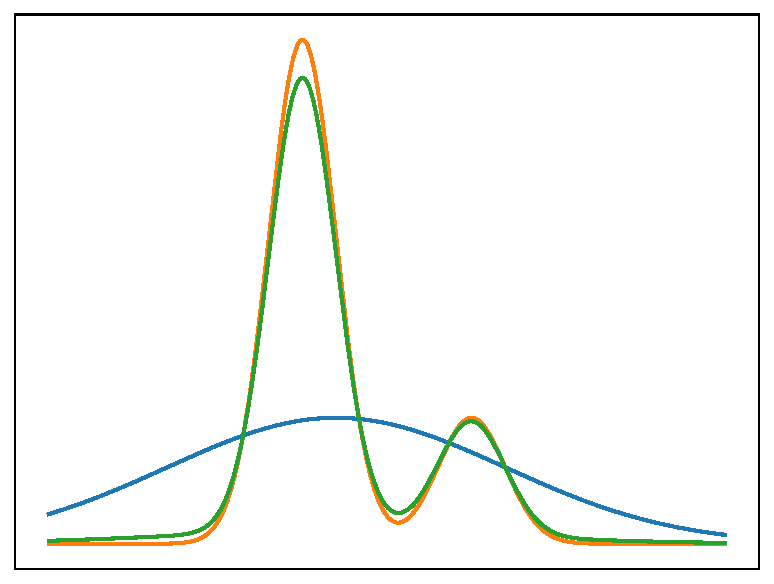
\includegraphics[width = .29\textwidth]{include/figures/1dplotslw100_delta1}
        & 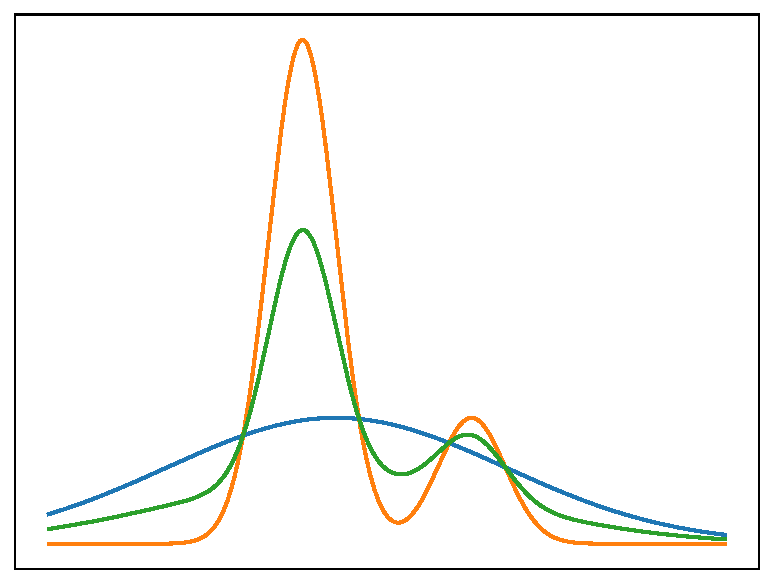
\includegraphics[width = .29\textwidth]{include/figures/1dplotslw100_delta5}
        & 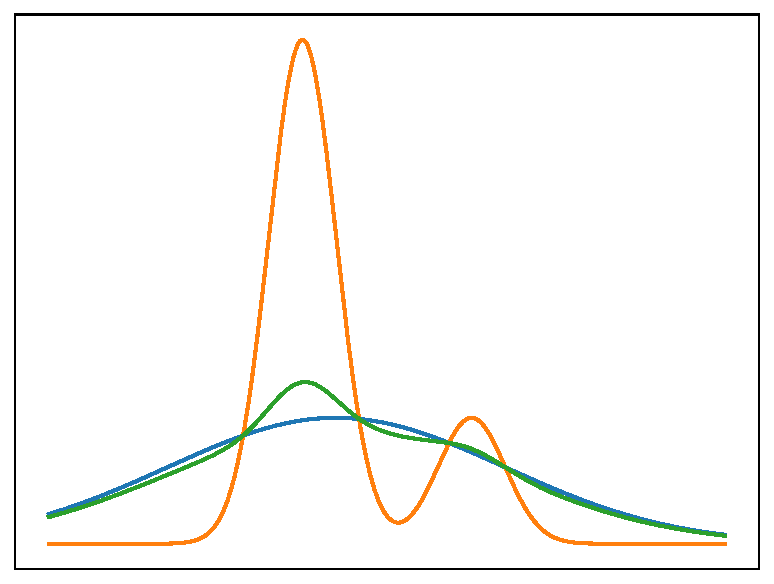
\includegraphics[width = .29\textwidth]{include/figures/1dplotslw100_delta9}
    \end{tabularx}
    \caption{1D Plots for different $\delta$ and $\sigma_{w3}$}
    $w_1 = 5$, $w_2 = -5$, $\alpha = 0.2$, $\sigma_w = 2$.
    The blue plot represents the third normal,
    the orange/red one represents the binormal,
    and the green one represents the mixture.
    The $x$ and $y$ labels and ticks are omitted for clarity.
    \label{tab:1dplotbitri}
\end{table}
\Cref{tab:1dplotbitri} offers a visual representation of how the parameter $\delta$ influences
the shape of the trinormal distribution.
Each plot illustrates \glspl{pdf} for different combinations of $\sigma_{w 3}$
(standard deviation of the third normal distribution) and $\delta$.
The row values in the table correspond to $\sigma_{w 3}$,
while the column values represent $\delta$.
We can observe two key trends within these plots:
\begin{enumerate}
    \item \emph{Influence of $\sigma_{w3}$:}
    As expected, varying $\sigma_{w3}$ primarily affects the \enquote{width}
    or overall variance of the combined distribution.
    When $\sigma_{w3}$ is larger than the width of the original binormal sum (orange/red line),
    choosing a larger $\delta$ allows the overall variance to increase significantly,
    as predicted by \cref{eq:w_prime_2_transform}.

    \item \emph{Decreasing skewness with increasing $\delta$:}
    The plots also reveal a distinct relationship between $\delta$
    and the skewness of the resulting distribution.
    As $\delta$ increases,
    the skewness of the combined trinormal distribution (green line) progressively reduces.
    This phenomenon can be attributed to the placement of the third normal distribution.
    Placed directly between the two original normal distributions,
    the third normal distribution acts as a centralizing force.
    As the weight of the third normal distribution (controlled by $\delta$) grows,
    its symmetric nature counteracts the potential skewness of the initial binormal sum.
    This effect is particularly strong in the bottom three plots,
    where a larger value of $\sigma_{w 3} = 10$ is used.
    We observe a clear reduction in the skewness of the green plot (mixture) as $\delta$ approaches 1.
\end{enumerate}
